% \documentclass[bwprint]{cumcmthesis} %去掉封面与编号页
\documentclass[withoutpreface,bwprint]{cumcmthesis} %去掉封面与编号页
\newcommand{\diff}{\mathop{}\!\mathrm{d}} % 正体微分符号

\usepackage{graphicx}       % 用于插入图片
\usepackage{subcaption} 
\usepackage{algorithm}
\usepackage{algorithmic} % 导言区需添加这两个宏包
\usepackage{comment}  

\usepackage{booktabs}
\usepackage{tabularx}
\usepackage{float}
\usepackage[numbers]{natbib}

\title{基于长短期记忆网络(LSTM)的蔬菜补货与定价决策模型}
\tihao{A}
\baominghao{1234}
\schoolname{XX大学}
\membera{yby}
\memberb{hyx}
\memberc{ssh}
\supervisor{老师}
\yearinput{2025}
\monthinput{08}
\dayinput{29}


\begin{document}

% 标题
\maketitle
\nocite{*}
\bibliographystyle{gbt7714-numerical}

\begin{abstract}
本文

    \textbf{针对问题一,}
你好

    \textbf{针对问题二,}

    \textbf{针对问题三,}

    \textbf{针对问题四,}

    \keywords{'xx'\quad'xx'\quad'xx'\quad'xx'\quad'xx'}
\end{abstract}

% 问题背景与重述
\section{问题重述}

\subsection{问题背景}
"板凳龙",

\subsection{问题提出}
某一板凳龙

\textbf{问题1:}

\textbf{问题2:}

\textbf{问题3:}

% 问题分析
\section{问题分析}

\subsection{问题一分析}

\subsection{问题二分析}

\subsection{问题三分析}

% 模型假设
\section{模型假设}

\begin{enumerate}
    \item 无人机知道自己的编号。
    \item 无人机主动机发射信号有次序,不是同时发射。
    \item 无人机调整方向为任意的。
\end{enumerate}

% 符号说明
\section{符号说明}
\begin{table}[H]
    \centering
    \caption{模型核心符号说明}
    \label{表标签}
    \begin{tabular}{ccc} 
        \toprule[1.5pt]
        \textbf{符号} & \textbf{说明} & \textbf{单位} \\
        \midrule[1pt]
        $g$ & 品类标识 & - \\
        $n_g$ & 第$g$类品类的样本量 & - \\
        \bottomrule[1.5pt]
    \end{tabular}
\end{table}

% 模型建立与求解
\section{模型建立与求解}
\subsection{问题一:建立被动接收信号无人机
的定位模型}


根据题意,先以FY00作为圆心,FY00与FY01连线方向为极轴,逆时针为正方向建立极坐标。在该极坐标下进行几何求解,位于圆心的无人机FY00和编队中另 2 架无人机发射信号,由于圆上第一架无人机选取具有任意性,为简化模型,方便计算,以FY01为一架主动机,选取其他任意一架无人机作为主动机,发射信号的无人机位置无偏差且编号已知,可由此确定被动机的位置。

\subsubsection{被动机定位模型建立}

根据我们建立的极坐标系,$R$为九架无人机分布圆的半径,可知FY00和FY01的极坐标分别为$(0,0)$,$(R,0)$,设另一架主动机$i$的极坐标为$(R,\theta)$,其中$\theta$已知,设接收信号的被动机$j$极坐标为$(r,\varphi)$,其中$(r)$与$(\varphi)$均未知。根据题意可知接收信号的被动机位置有如下两种情况:

\begin{enumerate}
    \item 当$\theta>\varphi$时,无人机分布的其中一种情况如图\ref{q1_1}所示,

    由几何关系可得
    \begin{equation}
    \left\{
    \begin{aligned}
        \frac{R}{\sin\alpha} &= \frac{r}{\sin(\pi - \alpha - \theta + \varphi)} \\
        \frac{R}{\sin\beta} &= \frac{r}{\sin(\pi - \varphi - \beta)}
    \end{aligned}
    \right.
    \end{equation}

    \item 当$\theta<\varphi$时,无人机分布的其中一种情况如图\ref{q1_2}所示,
    
    由几何关系可得
    \begin{equation}
    \left\{
    \begin{aligned}
        \frac{R}{\sin\alpha} &= \frac{r}{\sin(\pi - \alpha + \theta - \varphi)} \\
        \frac{R}{\sin\beta} &= \frac{r}{\sin(\pi - \varphi - \beta)}
    \end{aligned}
    \right.
    \end{equation}
    
\end{enumerate}


$\theta$与$\varphi$的取值范围有$\theta \in[0,\pi)\cap \varphi \in[0,\pi)$,$\theta \in[0,\pi)\cap \varphi \in[\pi,2\pi)$,$\theta \in[\pi,2\pi)\cap \varphi \in[0,\pi)$,$\theta \in[\pi,2\pi)\cap \varphi \in[\pi,2\pi)$四种情况。易证$\theta$与$\varphi$的取值范围不影响数值解的大小,仅影响解的正负,故仅从$\theta$与$\varphi$的大小关系出发进行讨论。上述描述便以$\theta \in[0,\pi]\cap \varphi \in[0,\pi)$为例,其他情况均同理。

\begin{figure}[htbp]
    \centering
    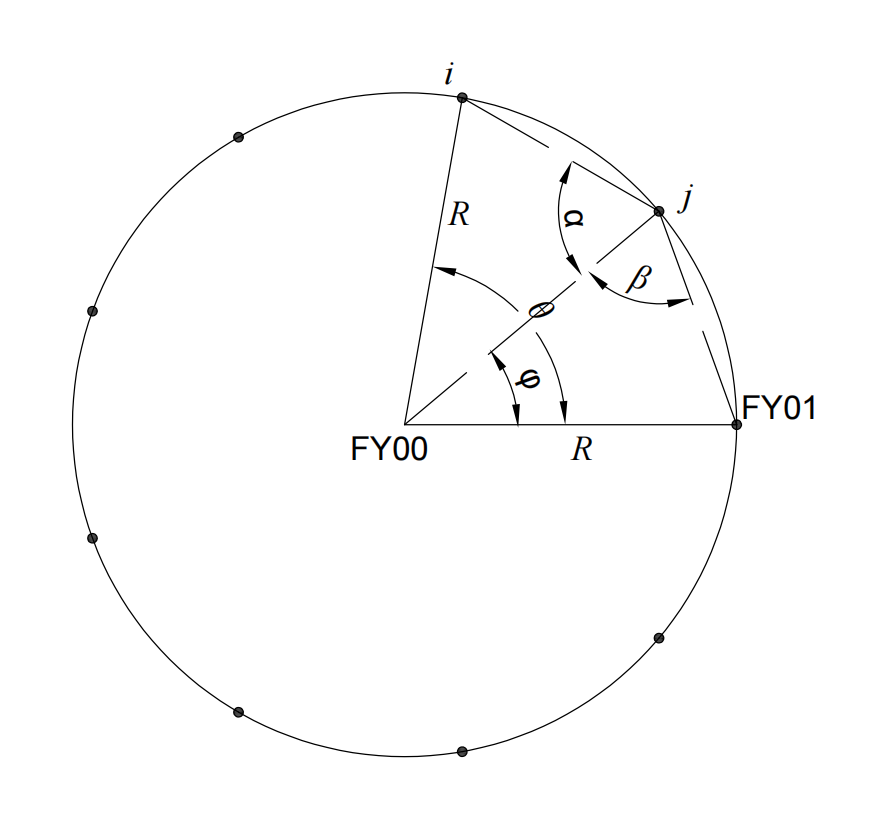
\includegraphics[width=0.5\textwidth]{../../figure/q1_1.png} 
    \caption{主动机与被动机排布的情况1}
    \caption*{\small 注:主动机发射的方向信息$\alpha$为$(i,0)$的夹角,$\beta$为$(0,1)$的夹角,图\ref{q1_2}同理。}
    \label{q1_1}
\end{figure}

\begin{figure}[htbp]
    \centering
    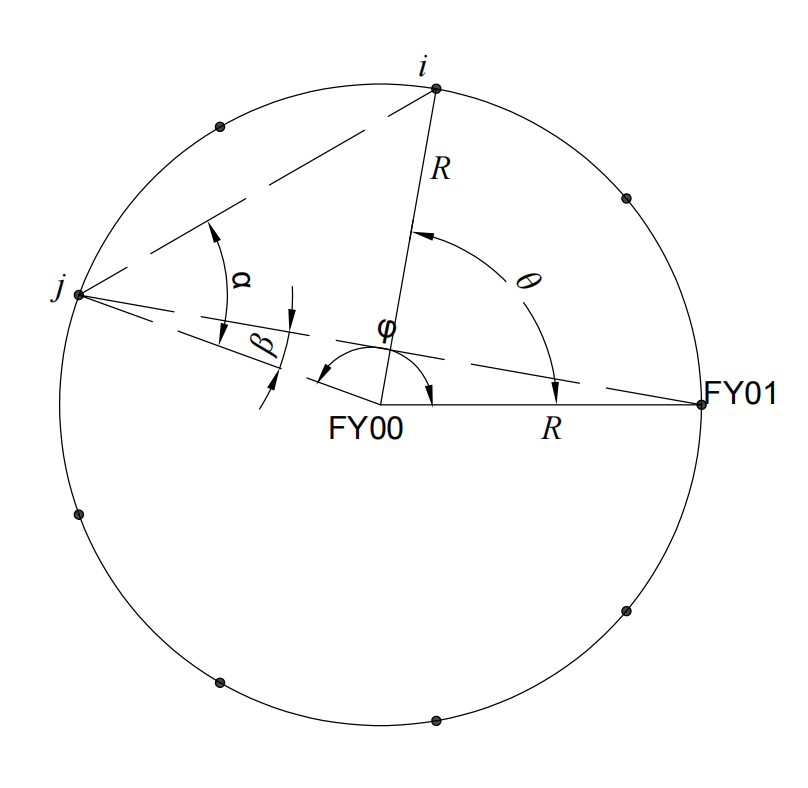
\includegraphics[width=0.5\textwidth]{../../figure/q1_2.png} 
    \caption{主动机与被动机排布的情况2}
    \label{q1_2}   
\end{figure}


\subsubsection{被动机定位模型求解}

将式\










\begin{figure}[htbp]
    \centering
    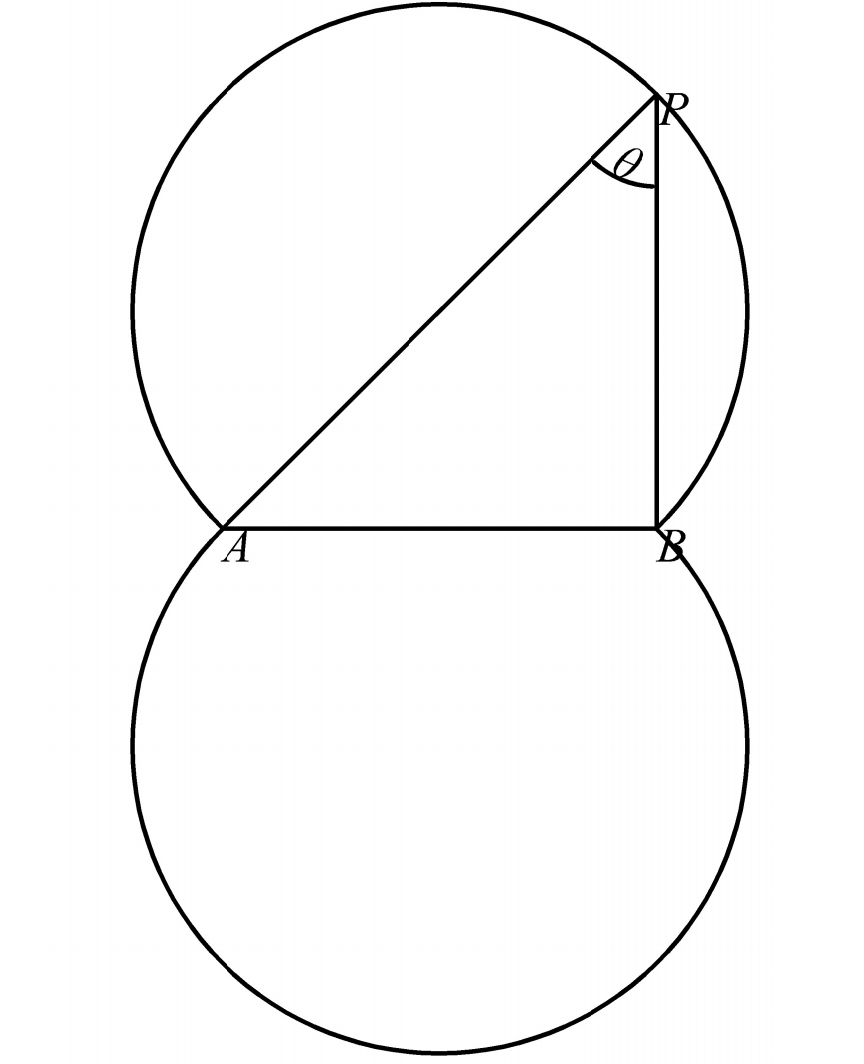
\includegraphics[width=0.5\textwidth]{../../figure/q1_3.png} 
    \caption{哈哈}  
    \label{q1_4}    
\end{figure}

\begin{figure}[htbp]
    \centering
    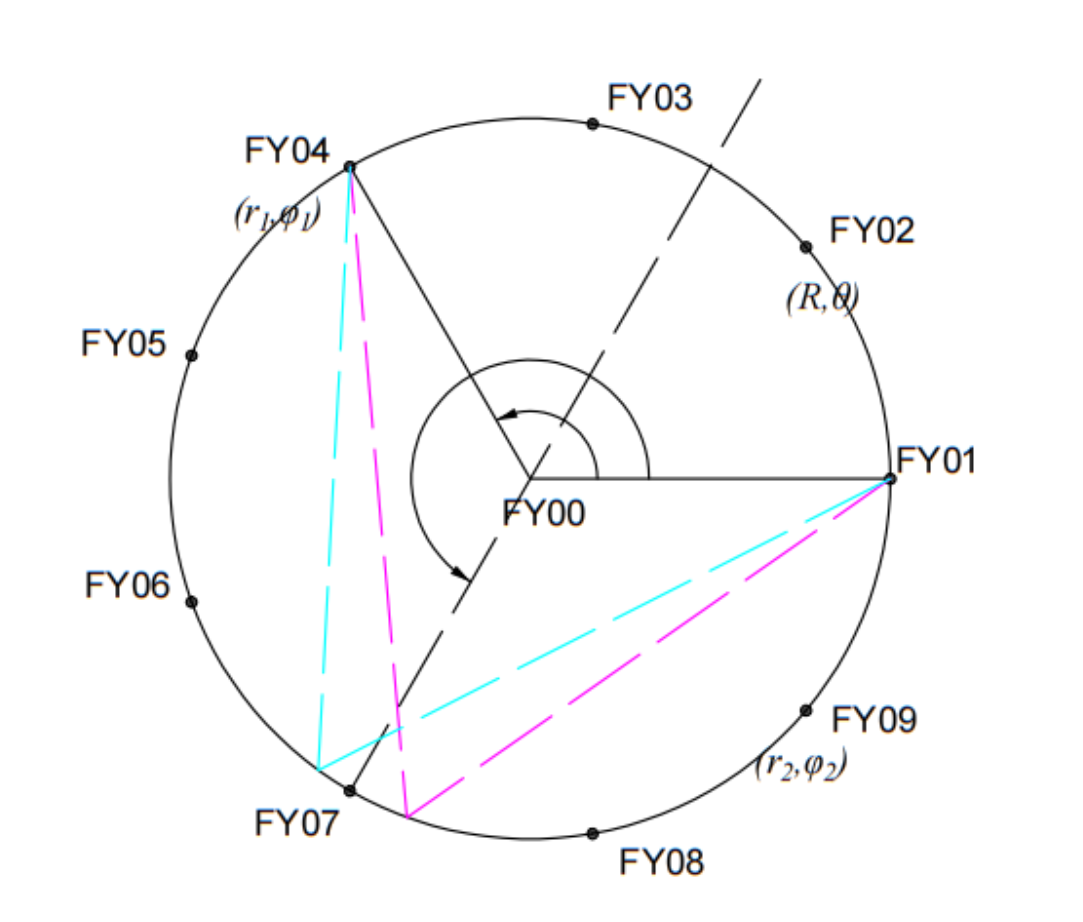
\includegraphics[width=0.5\textwidth]{../../figure/q1_4.png} 
    \caption{哈哈}
    \label{q1_3}   
\end{figure}

\subsubsection{问题求解}
\subsubsection{求解结果}

\subsection{问题二的模型建立与求解}
\subsubsection{模型建立}
\subsubsection{问题求解}
\subsubsection{求解结果}

\subsection{问题三的模型建立与求解}
\subsubsection{模型建立}
\subsubsection{问题求解}
\subsubsection{求解结果}

% 模型的分析与检验
\section{模型的分析与检验}
\subsection{误差分析}
\subsection{灵敏度分析}


% 模型评价
\section{模型的评价}
\subsection{模型优点}
\begin{enumerate}
    \item ..
    \item ..
    \item ..
\end{enumerate}

\subsection{模型缺点}
\begin{enumerate}
    \item ..
    \item ..
\end{enumerate}

\subsection{改进方向}
\begin{enumerate}
    \item ..
    \item ..
\end{enumerate}

% 摘要
\bibliography{ref}

% 附录

\begin{appendices}

\section{运行结果}


\section{文件列表}
\begin{table}[H]
    \caption{程序文件列表}
    \centering
    \begin{tabularx}{\textwidth}{l X}
        \bottomrule
        文件名 & 功能描述 \\
        \midrule
        Enums.py & 自定义枚举类型 \\
        SaleFlow.py & 处理文档,将附件2的流水整理为便用的形式 \\
        SaleUtils.py & 处理表格、绘图等工具 \\
        code1.py & 问题一程序代码 \\
        code2.py & 问题二程序代码 \\
        code3.py & 问题三程序代码 \\
        \bottomrule
    \end{tabularx}
    \label{tab:文件列表}
\end{table}

\section{代码}
问题1代码
\lstinputlisting[language=python]{../../code/code1.py}
问题2代码
\lstinputlisting[language=python]{../../code/code2.py}
问题3代码
\lstinputlisting[language=python]{../../code/code3.py}

\end{appendices}

\end{document}